\section{DiaTrend Dataset}
\label{sec:eda_diatrend}

\subsection{Dataset Description}
\label{subsec:diatrend_dataset_description}

The dataset includes both a patient-level information table that provides demographic information, and a glucose measurement table with the timestamped glucose values.

The patient information table includes the following variables: patient identifier (\verb|patient_id|), sex (\verb|sex|), age (\verb|age|), number of days with measurements (\verb|measurement_days|), and total number of measurements (\verb|measurement_count|).

The glucose measurement table includes the following variables: patient identifier (\verb|patient_id|), measurement date (\verb|date|), measurement time (\verb|time|), glucose value (\verb|glucose|), and temporal alignment columns at 5-minute and/or 15-minute resolution (\verb|timestamp_5min| and \verb|timestamp_15min|).

\begin{table}[htbp]
    \centering
    \caption{General description of the DiaTrend dataset.}
    \label{tab:diatrend_general_description}
    \begin{tabular}{ll}
        \hline
        \textbf{Metric} & \textbf{Value} \\
        \hline
        Number of patients & 51 \\
        Total number of glucose measurements & 7,667,356 \\
        \hline
        Start date & 2015-12-01 21:01:07 \\
        End date & 2022-06-28 23:59:34 \\
        Total recording span & 2,401 days \\
        Number of days with measurements & 2,358 \\
        \hline
        Rows with 5-minute alignment & 8,750,125 \\
        Rows with 15-minute alignment & 2,916,712 \\
        \hline
    \end{tabular}
\end{table}

Additionally, a consistency check was performed between the patient metadata table and the measurements table. Although the metadata file contains information for 54 patients, only 51 patients are present in the measurement dataset. Specifically, patients 50, 52, and 54 appear in the metadata table but do not have associated glucose measurements in the processed dataset. Therefore, analysis will be based on the 51 patients for whom glucose records are available on the measurements table.

\begin{table}[htbp]
    \centering
    \caption{Patient information summary for the DiaTrend dataset.}
    \label{tab:diatrend_patient_information}
    \begin{tabular}{ll}
        \hline
        \textbf{Metric} & \textbf{Value} \\
        \hline
        Mean age & 30.57 \\
        Median age & 25 \\
        Minimum age & 19 \\
        Maximum age & 69 \\
        \hline
        Male patients & 16 \\
        Female patients & 35 \\
        \hline
        Mean days with measurements per patient & 540 \\
        Median days with measurements per patient & 261 \\
        \hline
        Mean measurements per patient & 150,340\\
        Median measurements per patient & 80,488 \\
        \hline
    \end{tabular}
\end{table}

This generic structural description provides the basic context needed for the following analyses

\subsection{Patient Contribution Analysis}
\label{subsec:diatrend_patient_contribution}

For each patient, the number of glucose measurements and the number of days with at least one measurement were computed and summarised in Table~\ref{tab:diatrend_patient_contribution}

\begin{table}[htbp]
    \centering
    \caption{Patient contribution summary for the DiaTrend dataset.}
    \label{tab:diatrend_patient_contribution}
    \begin{tabular}{ll}
        \hline
        \textbf{Metric} & \textbf{Value} \\
        \hline
        Mean measurements per patient & 150,340 \\
        Median measurements per patient & 80,488 \\
        Minimum measurements per patient & 9,075 \\
        Maximum measurements per patient & 475,992 \\
        \hline
        Mean days per patient & 540 \\
        Median days per patient & 261 \\
        Minimum days per patient & 33 \\
        Maximum days per patient & 1,907 \\
        \hline
        Percentage contributed by the largest patient & 6.21\% \\
        Percentage contributed by the top 5 patients & 29.32\% \\
        Percentage contributed by the top 10 patients & 53.27\% \\
        Number of patients contributing 50\% of the dataset & 10 \\
        \hline
    \end{tabular}
\end{table}

Figure~\ref{fig:measurements_per_patients_Diatrend} shows the number of measurements per patient, sorted in descending order.

\begin{figure}[htbp]
    \centering
    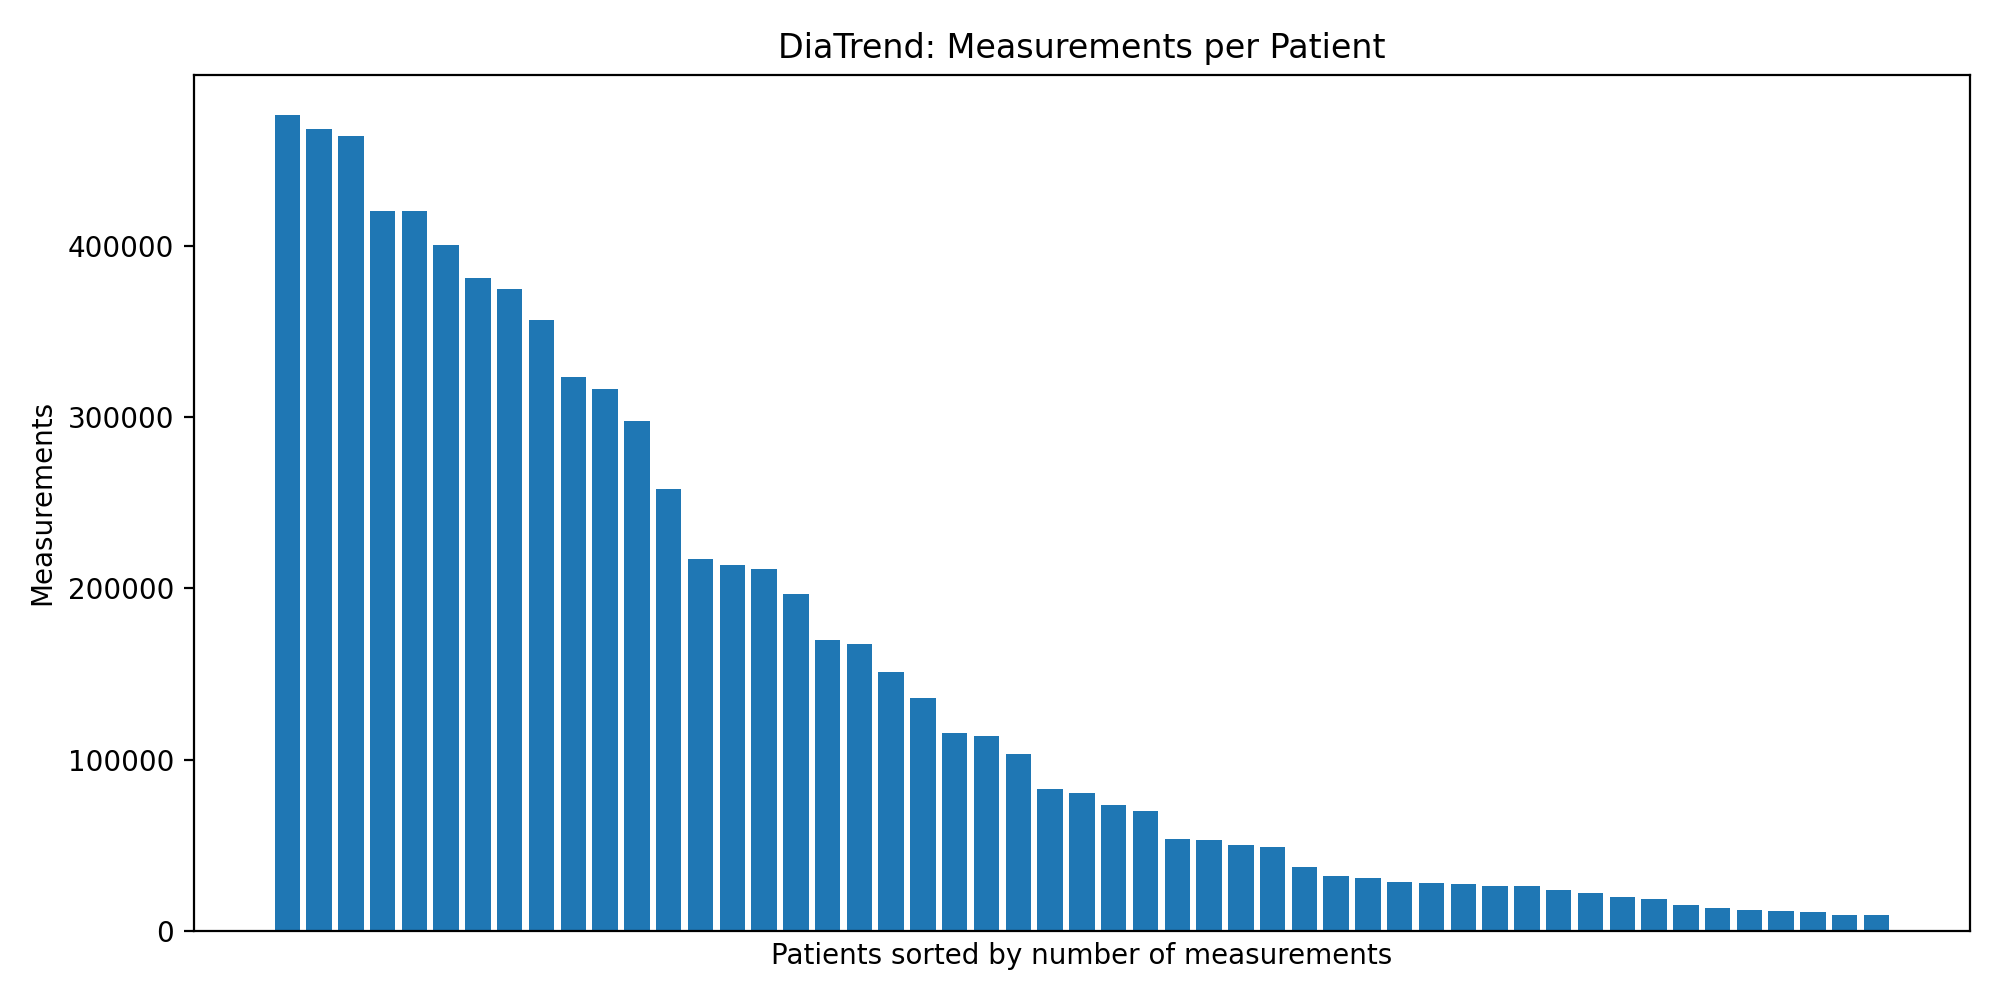
\includegraphics[width=1\textwidth]{images/EDA_Diatrend/measurements_per_patient.png}
    \caption{Measurements per patient in DiaTrend.}
    \label{fig:measurements_per_patients_Diatrend}
\end{figure}

In this dataset, patient contribution to the total glucose measurements distribution is highly uneven, as clearly shown by the descending pattern of Figure~\ref{fig:measurements_per_patients_Diatrend}.

Quantitatively, as shown in Table~\ref{tab:diatrend_patient_contribution}, the largest patient contributes 6.21\% of all measurements, while the top 5 patients account for 29.32\% and the top 10 patients account for 53.27\% of the dataset. In other words, approximately half of all available glucose measurements come from only 10 out of the 51 analyzed patients, which makes the global distribution highly influenced by the glycemic profiles of those individuals with the larger monitoring history. While this finding does not necessarily introduces a bias towards the scope of this thesis -- which is mostly agnostic to individual patient characteristics, it is still relevant enough to be taken into consideration for the subsequent analyses.

\subsection{Glucose Descriptive Statistics}
\label{subsec:diatrend_glucose_statistics}

This section provides a general view of the global distribution of glucose values.

\begin{table}[htbp]
    \centering
    \caption{Glucose descriptive statistics for the DiaTrend dataset.}
    \label{tab:diatrend_glucose_statistics}
    \begin{tabular}{ll}
        \hline
        \textbf{Metric} & \textbf{Value} \\
        \hline
        Minimum glucose & 39 mg/dL \\
        Maximum glucose & 401 mg/dL \\
        Mean glucose & 186.33 mg/dL \\
        Median glucose & 175 mg/dL \\
        Standard deviation & 74.18 mg/dL \\
        \hline
    \end{tabular}
\end{table}

\begin{figure}[htbp]
    \centering
    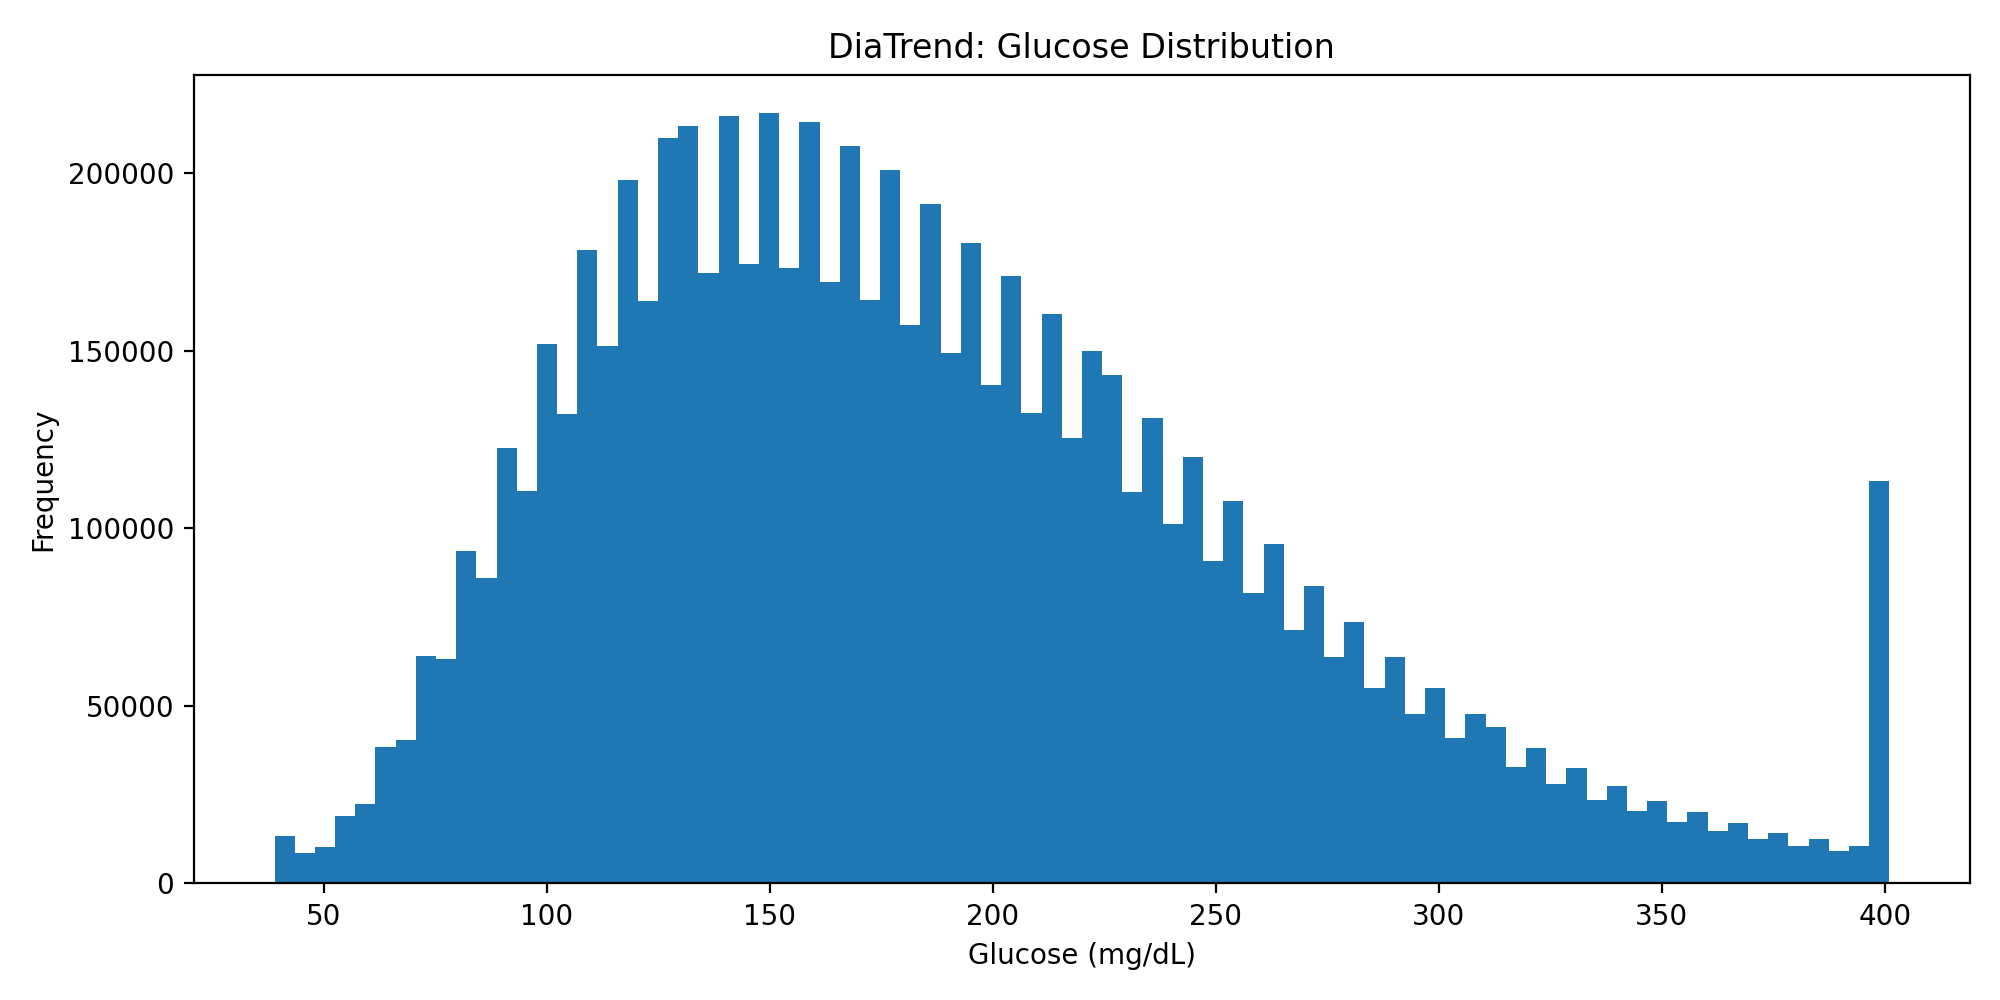
\includegraphics[width=1\textwidth]{images/EDA_Diatrend/glucose_distribution.png}
    \caption{Glucose distribution in DiaTrend.}
    \label{fig:glucose_distribution_Diatrend}
\end{figure}

As shown in Figure~\ref{fig:glucose_distribution_Diatrend}, the glucose distribution follows a typical diabetes-related pattern: the highest concentration of measurements appears around the central normoglycemic and early hyperglycemic regions, while the frequency gradually decreases towards the more extreme hypoglycemic and severe hyperglycemic values.

It is also interesting to note how the histogram presents an irregular pattern with alternating peaks and lower bars. This “one peak, one drop” effect may be related to the measurement resolution, rounding, or preprocessing of CGM values, but it does not change the general shape of the distribution.

\subsection{Glycemic-Range Distribution}
\label{subsec:diatrend_ranges_distribution}

While the previous section describes glucose distribution globally, this one focuses on the analysis of clinically relevant glycemic ranges. As for a reference, the following glycemic ranges are formally presented in Table~\ref{tab:glycemic_range_definitions}:

\begin{table}[htbp]
    \centering
    \caption{Glycemic range definitions.}
    \label{tab:glycemic_range_definitions}
    \begin{tabular}{ll}
        \hline
        \textbf{Glycemic range} & \textbf{Definition} \\
        \hline
        Severe hypoglycemia & $<54$ mg/dL \\
        Hypoglycemia & $54$--$69$ mg/dL \\
        Normoglycemia & $70$--$180$ mg/dL \\
        Hyperglycemia & $181$--$250$ mg/dL \\
        Severe hyperglycemia & $>250$ mg/dL \\
        \hline
    \end{tabular}
\end{table}

The count and the derived percentage of glucose measurements were computed for each of the previous ranges in Diatrend.

\begin{table}[htbp]
    \centering
    \caption{Glycemic range distribution in DiaTrend.}
    \label{tab:diatrend_glycemic_distribution}
    \begin{tabular}{lrr}
        \hline
        \textbf{Glycemic range or category} & \textbf{Count} & \textbf{Percentage} \\
        \hline
        Severe hypoglycemia & 35,291 & 0.46\% \\
        Hypoglycemia & 105,621 & 1.38\% \\
        Normoglycemia & 3,901,129 & 50.88\% \\
        Hyperglycemia & 2,192,705 & 28.60\% \\
        Severe hyperglycemia & 1,432,610 & 18.68\% \\
        \hline
        TBR ($<70$ mg/dL) & 140,912 & 1.84\% \\
        TIR ($70$--$180$ mg/dL) & 3,901,129 & 50.88\% \\
        TAR ($>180$ mg/dL) & 3,625,315 & 47.28\% \\
        \hline
    \end{tabular}
\end{table}

\begin{figure}[htbp]
    \centering
    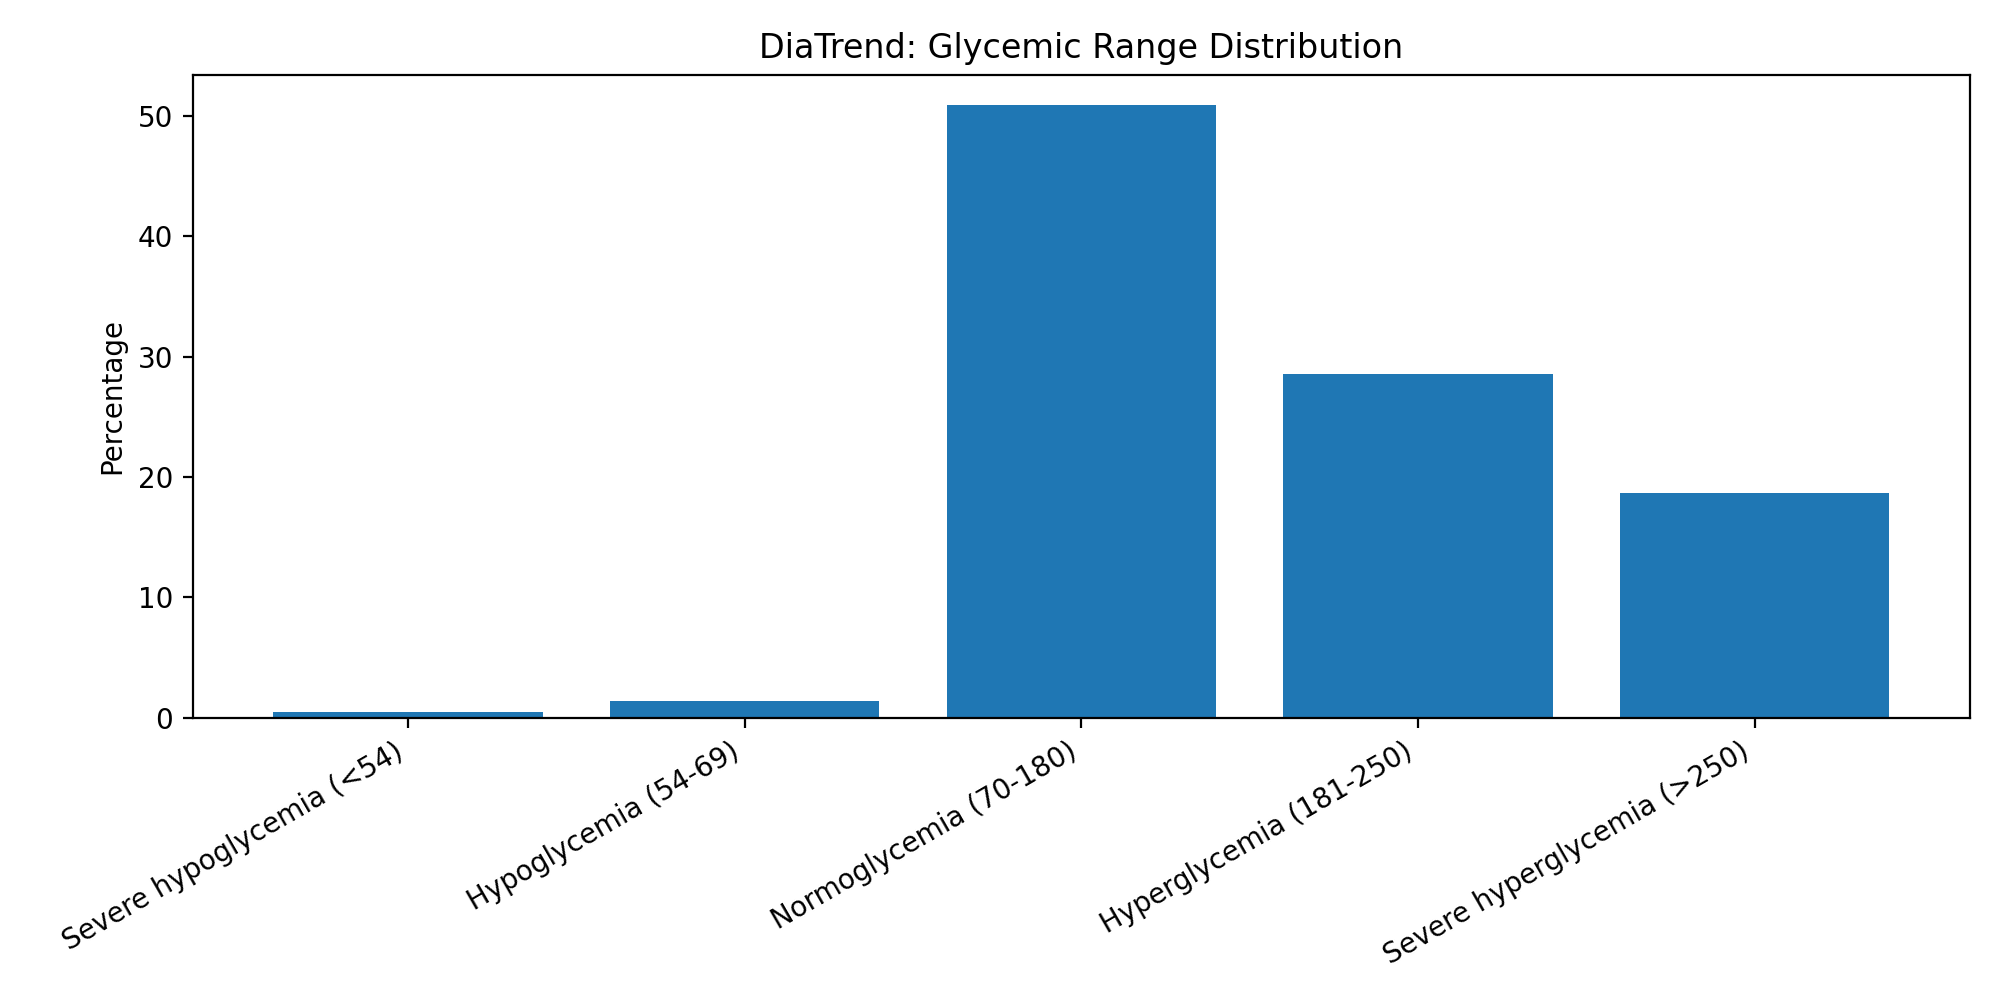
\includegraphics[width=1\textwidth]{images/EDA_Diatrend/glycemic_range_distribution.png}
    \caption{Glycemic range distribution}
    \label{fig:glycemic_range_distribution_Diatrend}
\end{figure}

Figure~\ref{fig:glycemic_range_distribution_Diatrend} makes the imbalance towards clinically critical glycemic ranges clearly visible. Quantitatively, as described in Table~\ref{tab:diatrend_glycemic_distribution}, normo-glycemia is the dominant range representing 50.88\% of all glucose values, hyperglycemia and severe hyperglycemia are also highly represented accounting together for the 47.28\% of the measurements, while hypoglycemia and severe hypoglycemia only account together for the 1.84\% of the total

\begin{table}[htbp]
    \centering
    \caption{Imbalance ratios in DiaTrend.}
    \label{tab:diatrend_imbalance_ratios}
    \begin{tabular}{lr}
        \hline
        \textbf{Ratio} & \textbf{Value} \\
        \hline
        Normoglycemia / hypoglycemia & 27.68 \\
        Normoglycemia / severe hypoglycemia & 110.54 \\
        Normoglycemia / hyperglycemia & 1.78 \\
        Normoglycemia / severe hyperglycemia & 2.72 \\
        Majority range / smallest minority range & 110.54 \\
        \hline
        TIR / TBR & 27.68 \\
        TIR / TAR & 1.08 \\
        \hline
    \end{tabular}
\end{table}

Additionally, the specific imbalance ratios where also quantified in Table~\ref{tab:diatrend_imbalance_ratios}, in order to express the imbalance in more direct quantitative terms, that is: "how much more frequent the majority ranges are compared the clinicall critical ones". For example, in DiaTrend, normoglycemic samples appear 27.68 times more frequently than hypoglycemic samples and 110.54 times more frequently than severe hypoglycemic samples.

\subsection{Patient-Level Glycemic Distribution}
\label{subsec:diatrend_patient_level}

While the global glycemic percentages presented in the previous section are useful, they may hide patient-level differences. For this reason, in order to make a more representative analysis of all the patients, the glycemic ranges distribution was also computed independently for each of them. A summarized version of theses results is presented in Table~\ref{tab:diatrend_patient_glycemic_statistics}

\begin{table}[htbp]
    \centering
    \caption{Patient-level glycemic range statistics in DiaTrend.}
    \label{tab:diatrend_patient_glycemic_statistics}
    \begin{tabular}{lr}
        \hline
        \textbf{Metric} & \textbf{Value} \\
        \hline
        Mean patient TBR & 1.67\% \\
        Median patient TBR & 1.18\% \\
        Minimum patient TBR & 0.06\% \\
        Maximum patient TBR & 9.31\% \\
        \hline
        Mean patient TIR & 53.97\% \\
        Median patient TIR & 52.52\% \\
        Minimum patient TIR & 16.03\% \\
        Maximum patient TIR & 79.57\% \\
        \hline
        Mean patient TAR & 44.36\% \\
        Median patient TAR & 46.50\% \\
        Minimum patient TAR & 18.96\% \\
        Maximum patient TAR & 83.87\% \\
        \hline
    \end{tabular}
\end{table}

\begin{figure}[htbp]
    \centering
    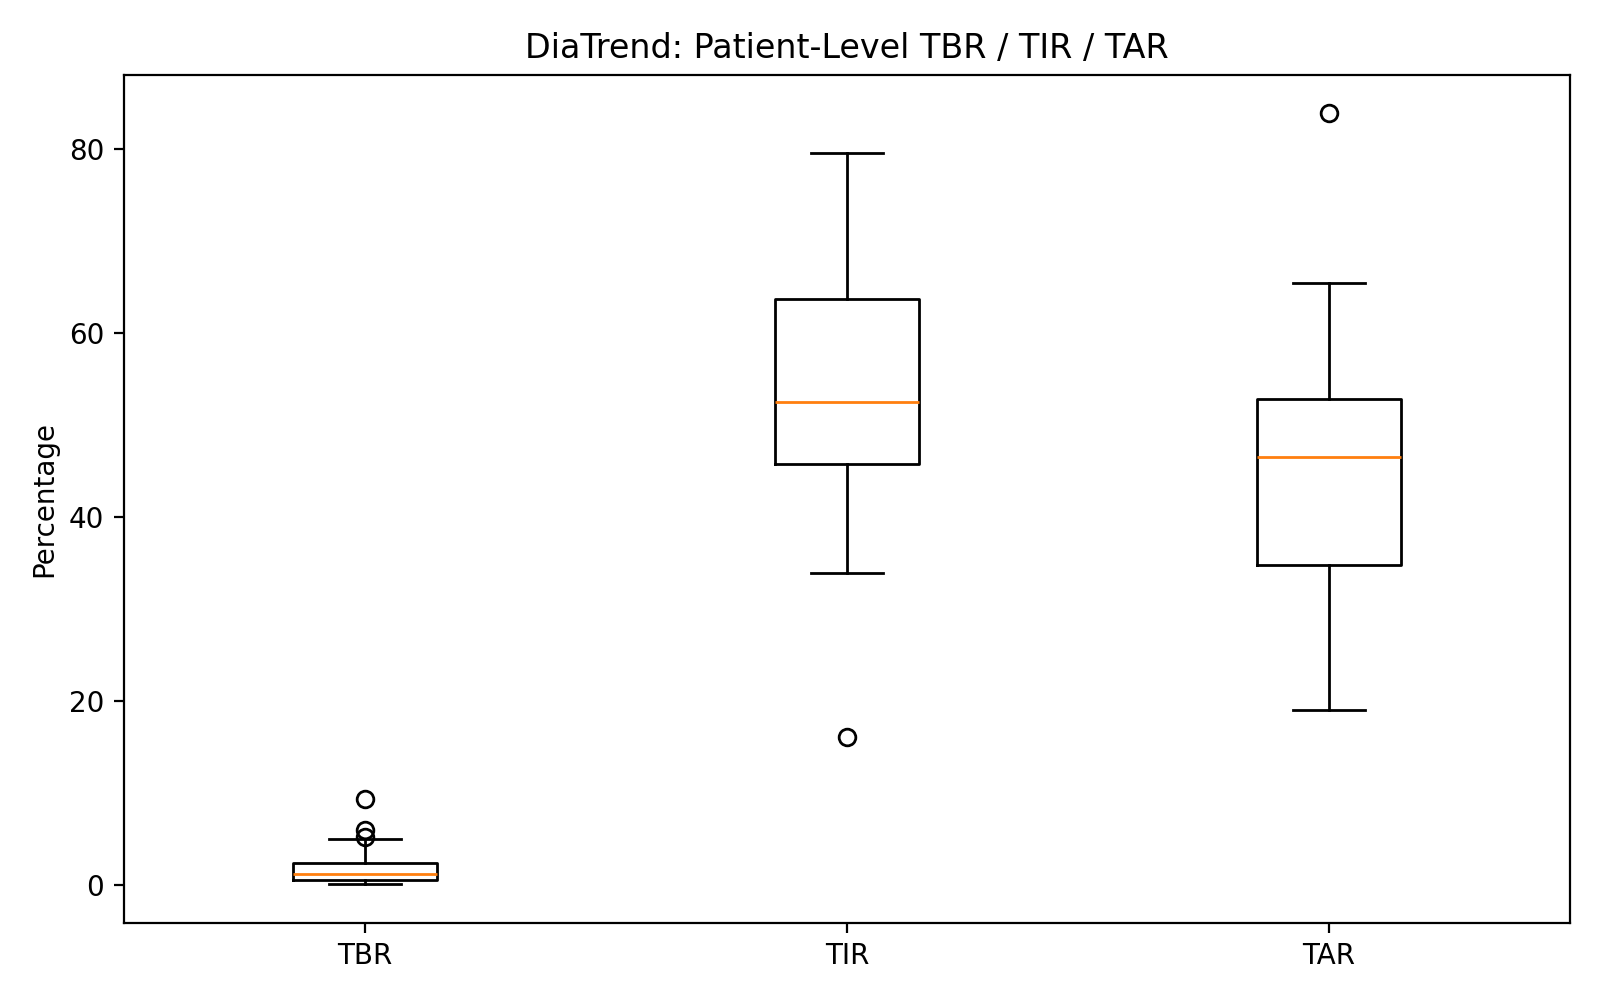
\includegraphics[width=1\textwidth]{images/EDA_Diatrend/patient_level_tbr_tir_tar.png}
    \caption{Glucose distribution in DiaTrend.}
    \label{fig:patient_boxplot_diatrend}
\end{figure}

Figure~\ref{fig:patient_boxplot_diatrend} makes patient-level distribution much more interpretable by presenting it in the form of a box-plot: each box summarises how each of ranges varies for the different patients. This representation allows to interpret whether the imbalance ratios described in general terms are actually equivalent for each patient of the dataset population.

The TBR boxplot is concentrated very close to zero, with a median of 1.18\% and a maximum value of 9.31\%. This indicates that hypoglycemic measurements are mostly consistently rare for most patients, not only at global dataset level. On the contrary, TIR and TAR show much wider variability: TIR has a median of 52.52\%, but ranges from 16.03\% to 79.57\%, while TAR has a median of 46.50\% and ranges from 18.96\% to 83.87\%. Therefore, although TIR is the majority range for 48 out of 51 patients, the balance between normoglycemia and hyperglycemia may vary substantially between different patients. In any case, the plot confirms the consistent under-representation of hypoglycemic values across patients, while normo and hyper-glycemia depends more on the patient.

\subsection{Summary of Findings}
\label{subsec:diatrend_summary}

DiaTrend contains 51 patients and 7,667,356 valid glucose measurements. The dataset covers the period from 2015-12-01 21:01:07 to 2022-06-28 23:59:34, with a total recording span of 2,401 days.

The patient contribution analysis shows that DiaTrend is highly uneven in terms of per-patient measurements availability. The largest patient contributes 6.21\% of all measurements, while the top 10 patients account for 53.27\% of the dataset.

The glucose distribution analysis shows a normo-diabetes pattern: the highest concentration of measurements appears around the central normoglycemic and early hyperglycemic regions, while the frequency gradually decreases towards the more extreme hypoglycemic and severe hyperglycemic values.

The imbalance ratios confirm this pattern quantitatively: normoglycemic samples appear 27.68 times more frequently than hypoglycemic samples and 110.54 times more frequently than severe hypoglycemic samples, while hyperglycemia and severe hyperglycemia appear together globally almost as much as normoglycemia.

At patient level, TBR remains consistently low across patients, which confirms that hypoglycemia is not only globally rare but also generally underrepresented across population. On the other hand, TIR and TAR show wider variability, indicating that the balance between normoglycemia and hyperglycemia highly depends on patient's characteristics.